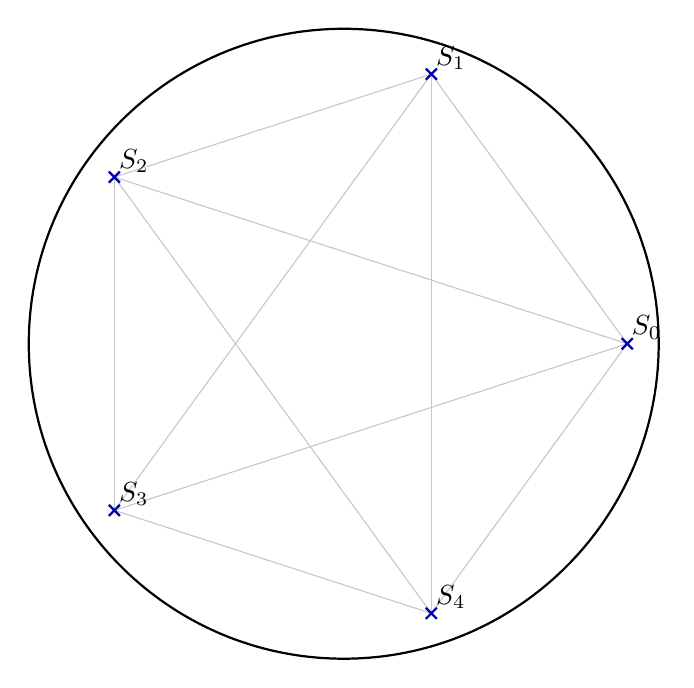
\begin{tikzpicture}[x=4cm,y=4cm]
  \draw[thick] (0,0) circle (1);
  \foreach \k in {0,...,4} {
    \coordinate (p\k) at ({72*\k}:.9);
  }
  \foreach \i in {0,...,4} {
    \foreach \j in {0,...,4} {
      \ifnum\i<\j
        \draw[black!22] (p\i)--(p\j);
      \fi
    }
  }
  \foreach \k in {0,...,4} {
    \draw[blue!70!black,thick]
      ([shift={(-2pt,-2pt)}]p\k)--([shift={(2pt,2pt)}]p\k)
      ([shift={(-2pt,2pt)}]p\k)--([shift={(2pt,-2pt)}]p\k);
    \node[above right,inner sep=1.5pt] at (p\k) {$S_{\k}$};
  }
\end{tikzpicture}
